\renewcommand{\lastmod}{8. Oktober 2024}
\renewcommand{\chapterauthors}{Markus Lippitz}

\chapter{Quantisierung}





% 2. Photoelectric Effect
% Sim: Photoelectric Effect
% • This is a much harder topic for students than professors think. For details, see:
% www.colorado.edu/physics/EducationIssues/papers/McKagan_etal/photoelectric.pdf
% • Common student difficulties (many can be resolved with sim):
% - think voltage rather than light takes electrons off plate
% - think current increases with speed of electrons
% - can’t explain basic function of experiment
% - can’t explain classical model of light
% - can’t explain why PE experiment leads to photon model of light
% • A general problem that first appears here is that some students have no ability to think
% hypothetically and can’t separate what was expected classically from what really happens.


% 5. Atomic Spectra and Discharge Lamps
% Sim: Discharge Lamps
% • We teach spectra before the Bohr model in order to emphasize how Bohr was able to explain
% the observed spectra with his model.
% • Students often have trouble with the idea that the energy of light corresponds to the difference
% between the levels rather than the values of the levels. They need lots of explicit practice to
% get this distinction straightened out.
% • We get lots of questions about how the electron chooses which level to jump down to, and
% how it decides when to jump down. These questions are useful later for emphasizing why the
% Schrodinger model of the atom is better than the Bohr model.
% • The simulation and associated homework really help students build a clear model of how a
% discharge lamp work. The one place they had trouble was relating this model to what they
% see in a real discharge lamp, even though we did a demo with real discharge lamps and
% diffraction gratings. It’s important to be really explicit in this demo about how the physical
% lamps relate to the model in the sim.
% • When reminding students of Coulomb potential energy, they remember the equation kq1q2/r,
% but often don’t realize that this is the same as –ke²/r.
% • The idea of how fluorescent lights work is harder for students than you might think because
% they have trouble with the idea that red+blue+green light l



% 7. Balmer Series
% • We emphasize the point that Balmer came up with his formula by playing around with
% numbers and didn’t know what it meant. This is probably lost of students who think all of
% physics is like that.


% 8. Bohr and deBroglie Models of the atom
% Sim: Models of The Hydrogen Atom
% • For details about why and how we teach this topic, see:
% www.colorado.edu/physics/EducationIssues/papers/McKagan_etal/BohrModel_McKagan_etal.pdf
% • This is really an opportunity to teach modeling and the significance of Bohr explaining where
% Balmer’s equation came from and deBroglie explaining why there are fixed energy levels.
% This is a really difficult section for students who have trouble thinking hypothetically.
% • In the Bohr model, students often mix up total and potential energy, for example, thinking
% that -13.6eV is the potential energy. This confusion is confounded by the way the total
% energy lines are drawn on top of the potential energy curves.


\section{Überblick}

Verschiedene Experimente haben gezeigt, dass die Energie eines Atoms oder eines Lichtstrahls \emph{quantisiert} ist, d.h. nur diskrete, wohldefinierte Werte annehmen kann. Die allermeisten Energien sind nicht möglich. In diesem Kapitel diskutieren wir diese Experimente und interpretieren ihre Ergebnisse:
\begin{itemize}
    \item Der \emph{Photoeffekt}, also das Herauslösen einzelner Elektronen aus einem Metall durch Licht, ist der zentrale Schritt zur Quantenhypothese des Lichts. Für seine Erklärung erhielt Einstein den Nobelpreis.
    \item Historisch gesehen hatte bereits Max Planck die Quantisierung eingeführt, um die \emph{Schwarzkörperstrahlung} zu erklären.
    \item Über Louis de Broglie kommen wir zu den \emph{Materiewellen}, also zu einer wellenartigen Beschreibung von Objekten, die wir sonst als Teilchen auffassen.
    \item Schließlich verwenden wir diese Materiewellen im \emph{Bohrschen Atommodell}, um endlich das Wasserstoffspektrum zu erklären.
\end{itemize}
Leider funktioniert das nur für Wasserstoff gut, so dass wir ein noch besseres Modell brauchen, was dann in den nächsten Kapiteln folgt.
Dieses Kapitel entspricht in seinem Aufbau dem Kapitel 38 von \cite{Knight_physics}. Gute andere Darstellungen finden sich in \cite{Haliday_Resnick}, \cite{Demtröder_ep3} und \cite{Haken_wolf_I}. Populärwissenschaftliche Darstellungen finde sich in \cite{QM100}
und \cite{QM_einstein}.


% Ich kann das Planck’sche Strahlungsgesetz herleiten und seinen Zusammenhang mit quantisierter Strahlung erklären. 

% Ich kann wichtige Versuche zur Quantisierung (Photoeffekt, Compton-Effekt, Frank-Herz-Versuch, Millikan-Versuch, Spektrallinien) erklären und darstellen, wie diese eine Quantenhypothese unterstützen. 

% Ich kann das Modell aus den Bohr’schen Postulaten herleiten, es in relevanten Fällen anwenden und seine Grenzen erklären.

\section{Der Photoelektrische Effekt}

Das zentrale und wichtige Experiment, das zur Quantenhypothese der Photonen führte, war der photoelektrische Effekt\sidenote{Auch Photoeffekt bzw. genauer äußerer Photoeffekt gennannt}. Bereits 1887 war bekannt, dass ultraviolettes Licht eine negativ geladene Platte eines Elektrometers entlädt, wobei Elektronen aus der Platte austreten.\sidenote{Diese austretenden Elektronen werden manchmal Photoelektronen genannt, sind aber völlig identisch mit allen anderen Elektronen.} Phillip Lenard hat dieses Experiment verfeinert. Die ehemals negativ geladene Platte bildet als Kathode zusammen mit einer Anode und einer Spannungsquelle einen Stromkreis. Die beiden Elektroden sind in einem Vakuumkolben eingeschlossen. Ein Gas spielt also keine Rolle. Wenn Licht auf die Kathode fällt, fließt ein Strom durch den Stromkreis, der gemessen werden kann. Dieser Strom muss also von den Elektronen getragen werden, die sich im Glaskolben von links nach rechts und damit im Uhrzeigersinn durch den Aufbau in Abbildung  \ref{fig:2_photoeffekt_setup} bewegen\phet{Photoelectric_Effect}
(technische Stromrichtung entgegen dem Uhrzeigersinn). Ohne Licht gibt es keine austretenden Elektronen und damit keinen Strom.

\begin{marginfigure}
    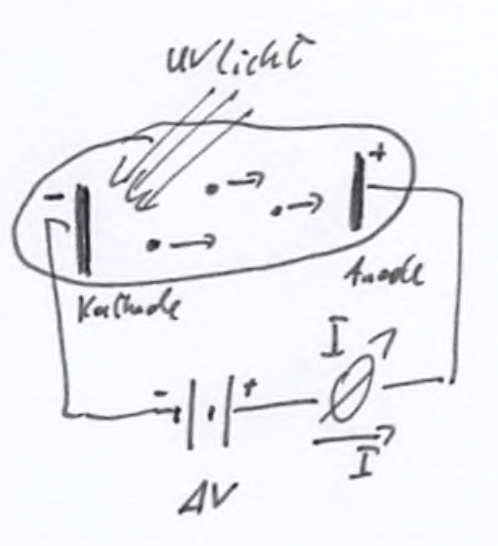
\includegraphics[width=\textwidth]{\currfiledir sketch/photoeffekt.png}
    \caption{Skizze des Versuchsaufbaus zum Photoeffekt}
    \label{fig:2_photoeffekt_setup}
\end{marginfigure}


Lenard untersuchte 1902 den Zusammenhang zwischen der Potentialdifferenz $\Delta V$ der Spannungsquelle und der Stromstärke $I$ im Stromkreis und den Einfluss der Lichtintensität und -frequenz $\nu = c / \lambda$. Er fand
\begin{enumerate}\setlength{\itemsep}{0pt}
    \item Der Strom $I$ ist proportional zur Lichtintensität.
    \item Es gibt keine Verzögerung zwischen dem Einschalten des Lichtes und dem Beginn des Stromflusses.
    \item Es gibt eine minimale Frequenz $\nu_0$ des Lichts, bzw. eine maximale Wellenlänge. Nur wenn das Licht diese Frequenz überschreitet (also blauer ist) fließt Strom. Dies kann nicht durch eine höhere Intensität kompensiert werden.
    \item Die minimale Frequenz $\nu_0$ hängt von der Art des Metalls in der Kathode ab.
    \item Die Stromstärke $I$ nimmt bei kleinen positiven Spannungen etwas zu. Bei großen Spannungen nimmt sie nicht mehr zu. Bei negativer Spannung wird die Stromstärke kleiner, bis bei einer Spannung $V = -V_{stop}$ kein Strom mehr fließt ($V_{stop}$ ist hier also als positiv definiert). 
    \item Diese Grenzspannung $V_{stop}$ ist unabhängig von der Lichtintensität. 
\end{enumerate}

\begin{marginfigure}
    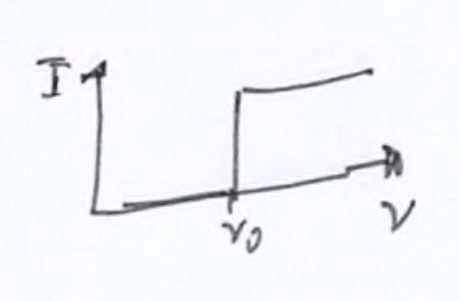
\includegraphics[width=0.6\textwidth]{\currfiledir sketch/PE_I_nu.png}
    \caption{Es gibt eine Grenzfrequenz $\nu_0$, unterhalb derer kein Strom detektiert wird.}
   \end{marginfigure}

   \begin{marginfigure}
    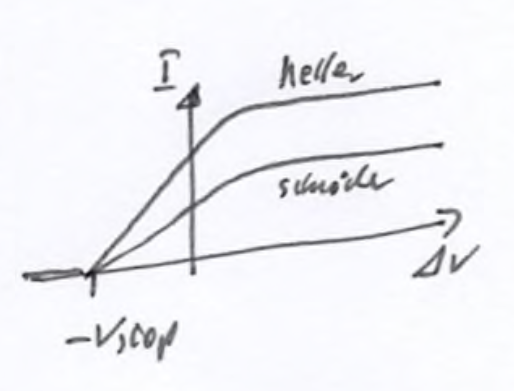
\includegraphics[width=\textwidth]{\currfiledir sketch/PE_I_V.png}
    \caption{Es gibt eine Stop-Spannung $- V_{stop}$,  unterhalb derer kein Strom detektiert wird.}
   \end{marginfigure}


Aus Sicht der klassischen Physik liefert die elektromagnetische Welle Energie, die im Metall in Form von Wärme gespeichert wird. Dies führt dazu, dass einige Elektronen die Austrittsarbeit überwinden und das Metall verlassen können. Dies wird als Glühemission bezeichnet und wurde beispielsweise in Röhrenfernsehgeräten genutzt.

Die Austrittsarbeit $W$ ist für jedes Metall unterschiedlich. Die meisten Metalle schmelzen, bevor eine nennenswerte Anzahl von Elektronen die Austrittsarbeit überwinden kann. Wolfram\sidenote{Schmelzpunkt 3422 °C, Austrittsarbeit 4.5 eV, mit Thorium 3.4 eV } besitzt eine geeignete Kombination aus Austrittsarbeit und hohem Schmelzpunkt und wird daher häufig als Glühwendel verwendet.

Einfache Berechnungen zeigen, dass die Energie eines Lichtstrahls auf zu viele Elektronen verteilt wird, so dass jedes Elektron sehr lange Energie sammeln müsste, um die Austrittsarbeit zu überwinden. Oder die Lichteinstrahlung konzentriert sich auf wenige Atome, die dann zu heiß werden. Es muss sich also beim Photoeffekt um etwas anderes als eine Glühemission handeln.

\subsection{Bedeutung der Stop-Spannung}

Welche Information kann aus der Stoppspannung $V_{stop}$ gewonnen werden? Die Austrittsarbeit $W$ ist die Energie, die mindestens aufgewendet werden muss, um ein Elektron aus dem Metall zu entfernen. Wird einem Elektron die Energie $E_{elec}$ zugeführt, so hat es außen maximal die Energie 
\begin{equation}
    E_{kin}^{max} = E_{elec} - W
\end{equation}
die allein in der Bewegung des Elektrons steckt. Die freigesetzten Elektronen haben also eine Geschwindigkeitsverteilung, deren obere Grenze durch die Austrittsarbeit $W$ bestimmt wird.

Je nach Potentialunterschied zwischen Kathode und Anode bewegen sich die austretenden Elektronen auf unterschiedlichen Bahnen. Eine positive Anode zieht Elektronen an. Mit zunehmender Anziehungskraft wandern auch Elektronen zur Anode, die sich ursprünglich in eine andere Richtung bewegt haben. Ab einer bestimmten Potentialdifferenz werden jedoch alle Elektronen gesammelt und der Strom erreicht einen Maximalwert.

Eine negative Anode stößt die Elektronen ab. Die Elektronen müssen gegen den Potentialberg laufen. Je negativer die Potentialdifferenz, d.h. je positiver $V_{stop}$, desto weniger Elektronen gelangen zur Anode. Die letzten Elektronen, die es noch zur Anode schaffen, sind die mit der maximalen kinetischen Energie, eben die mit $ E_{kin}^{max}$. Die Stoppspannung $V_{stop}$ ist also durch die Austrittsarbeit $W$ gegeben, wenn man die zugeführte Energie $E_{elec}$ kennt:
\begin{equation}
    V_{stop} = \frac{E_{kin}^{max}}{e} = \frac{E_{elec} - W}{e}  \quad .
\end{equation}
Dies nennt man darum Gegenfeldmethode.




\section{Klassische Deutung des Photoeffekts}

Aus Sicht der klassischen Physik ist Beobachtung 1, d.h. die Intensitätsabhängigkeit, gut erklärbar. Beobachtung 5 kann ebenfalls mit der Austrittsarbeit erklärt werden. Für die Grenzfrequenz $\nu_0$ des Lichts und die Tatsache, dass diese auch durch hohe Lichtintensitäten nicht verschoben werden kann, gibt es kein klassisches Modell. Auch die Stoppspannung sollte klassischerweise von der Lichtintensität und damit von der Temperatur der Elektronen abhängen. Schließlich kann, wie oben diskutiert, das sofortige Einsetzen des Stromflusses nicht klassisch erklärt werden.

\begin{questions}
    \item Schätzen Sie ab, wie groß die Energie pro Elektron wäre, wenn die Energie eines Lichtstrahls gleichmäßig auf alle Elektronen eines Metalls innerhalb der Eindringtiefe verteilt wäre.
    \item Schätzen Sie ab,  wie heiß ein Metall sein muss, damit eine nennenswerte Anzahl von Elektronen durch Glühemission freigesetzt wird.
\end{questions}

\section{Einsteins Quantenhypothese}

Im Jahr 1905, dem 'annus mirabilis',  veröffentlichte Albert Einstein 4 wichtige Artikel:
\begin{enumerate}\setlength{\itemsep}{0pt}
    \item Die Erklärung des photoelektrischen Effekts, die wir hier besprechen werden und für die er 1921 den Nobelpreis erhielt (\cite{Einstein05_licht}).
    \item Die Erklärung der Brownschen Bewegung mit der Diffusionskonstante $D = \mu k_b T$ (\cite{Einstein05_waerme}).
    \item Die spezielle Relativitätstheorie (\cite{Einstein05_ED})
    \item Die Masse-Energie-Äquivalenz mit $E = m c^2$ (\cite{Einstein05_energie})
\end{enumerate}

\begin{marginfigure}
    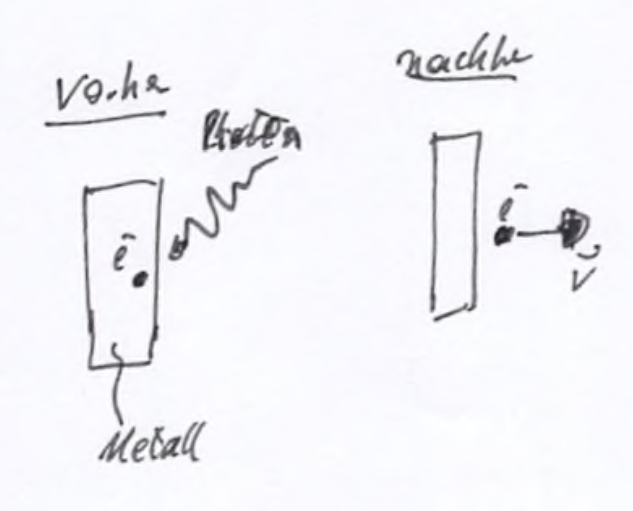
\includegraphics[width=\textwidth]{\currfiledir sketch/PE_Einstein.png}
    \caption{Ein Photon wird vernichtet und ein Elektron tritt aus dem Metall aus.}
\end{marginfigure}


Der entscheidende Punkt bei der Erklärung des Photoeffektes war die Annahme, dass die Energie einer Lichtwelle \emph{quantisiert} ist. Es gibt eine kleinste mögliche Energiemenge und alles andere sind ganzzahlige Vielfache davon. Dieses Lichtquantum nennt man heute \emph{Photon}. Es bewegt sich mit Lichtgeschwindigkeit.  Die Energie $E$ eines Photons hängt von der Frequenz $\nu$ der Lichtwelle ab
\begin{equation}
    E = h \, \nu \quad \text{mit} \quad h = 6,63 \cdot 10^{-34} \, J \, s = 4.14 \cdot 10^{-15}\, eV \, s
\end{equation}
mit der Planckschen Konstanten $h$. 

Neben dieser Annahme der Quantelung der Energie sind noch zwei weitere nötig: Die Absorption und Emission von Licht erfolgt immer in ganzen Quanten, die bei der Absorption vernichtet und bei der Emission erzeugt werden. Und die Energie wird immer auf genau ein Elektron übertragen, nicht auf mehrere.

\emph{Für diese Quantenhypothese gibt es keine klassische Entsprechung.} Wie wir sehen werden, reicht sie aber aus, um den Photoeffekt zu erklären.

Auf das Metall trifft Licht der Frequenz $\nu$. Jedes Photon hat dabei die Energie $E = h \nu$. Bei der Absorption wird diese Energie auf genau ein Elektron übertragen. Wenn sie ausreicht, um die Austrittsarbeit zu leisten ($h \nu > W$), kann das Elektron das Metall verlassen. Für die Grenzfrequenz des Lichtes gilt dann
 \begin{equation}
     \nu > \nu_0 = \frac{W}{h} \quad .
 \end{equation}
 Dies ist eine scharfe Grenze, wie im Experiment beobachtet.

 Höhere Lichtintensität bedeutet mehr Photonen, nicht Photonen mit höherer Energie. Es können also mehr Elektronen austreten, es kann mehr Strom fließen, aber nur, wenn die Grenzfrequenz überschritten wird, der Prozess also für ein einzelnes Photon ablaufen kann.

 Die Stoppspannung $V_{stop}$ ergibt sich aus der Energiedifferenz des Photons und der Austrittsarbeit, d.h. 
 \begin{equation}
     V_{stop} = \frac{h \nu - W}{e} \quad .
 \end{equation}
 Sie ist also insbesondere nicht von der Lichtintensität abhängig.

 \begin{marginfigure}
    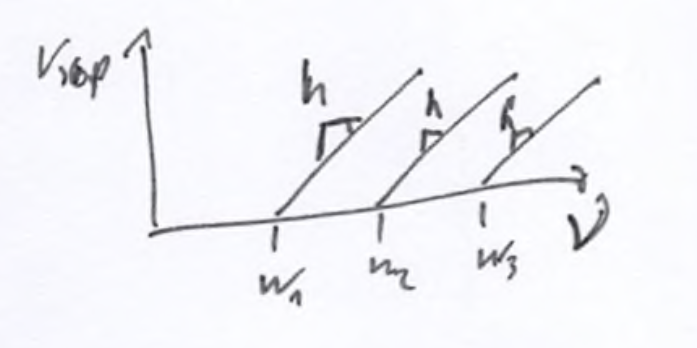
\includegraphics[width=\textwidth]{\currfiledir sketch/PE_Vstop.png}
    \caption{Stop-Spannung als Funktion der Frequenz $\nu$ für 3 verschiedene Metalle.}
\end{marginfigure}


 Schließlich ist die Absorption instantan. Das Elektron nimmt die Energie des Photons sofort auf, es kann sofort austreten und es gibt keine Zeitverzögerung zwischen dem Einfangen des Lichtes und dem Beginn des Stromflusses.

 Die Quantenhypothese von Albert Einstein kann also den Photoeffekt vollständig erklären. Sie gilt als Startschuss für die moderne Physik.

 \paragraph*{Nebenbemerkung} Auch nach unserer heutigen Überzeugung ist die Energie in einem Lichtstrahl in Photonen quantisiert, und auch alle anderen Annahmen finden heute noch Zustimmung. Wenn man aber genau ist, braucht man die Annahme der Quantisierung des \emph{Lichtfeldes} nicht zur Erklärung des Photoeffekts. Es genügt, dass das \emph{Elektron} der Quantenmechanik unterliegt. In den üblichen Vorlesungen und Büchern über Quantenmechanik wird das Elektron als quantenmechanisches Objekt mit Operatoren beschrieben, aber das Lichtfeld bleibt klassisch. Dies wird als '1. Quantisierung' bezeichnet und führt z.B. zu Fermis Goldener Regel, die auch den Photoeffekt beschreibt. Erst in der '2. Quantisierung' wird auch das Lichtfeld quantisiert und es werden Effekte beschrieben, die nur durch Photonen erklärt werden können, z.B. 'Anti-Bunching'.


 \section{Plancks Erklärung der Schwarzkörperstrahlung}

Hier reiche ich Max Plancks Erklärung der Schwarzkörperstrahlung nach. Er hat sie 1900 veröffentlicht und sie war die Grundlage für Einsteins Quantenhypothese. Max Planck nahm auch an, dass die Energie einer Lichtwelle gequantelt ist, ohne jedoch wirklich von Quanten als Objekten zu sprechen.

\subsection{Modendichte eines Resonators}

Zunächst müssen wir die Modendichte einführen und berechnen. Diese Art der Berechnung wird später in der Festkörperphysik an verschiedenen Stellen immer wieder vorkommen.

Wir betrachten einen verspiegelten quaderförmigen Hohlraum der Kantenlänge $L$. In ihm bilden sich wie in einem Resonator stehende Lichtwellen aus. Für die Wellenlänge $\lambda$ muss gelten
\begin{equation}
     L = n_x \frac{\lambda}{2} \quad \text{bzw} \quad k_x = \frac{2 \pi}{\lambda} = \frac{n_x \pi }{L}
\end{equation}
mit $n_x > 0$. Der Wellenvektor $\bk$ hat drei Komponenten
\begin{equation}
    k = | \bk | = \sqrt{k_x^2 + k_y^2 + k_z^2 } = \frac{\pi}{L} \sqrt{n_x^2 + n_y^2 + n_z^2} \quad .
\end{equation}
Im dreidimensionalen k-Raum sind die möglichen Werte von $\bk$ also die Punkte auf einem kubischen Gitter mit dem Abstand der Gitterpunkte $\pi / L$, wobei nur der positive Oktand erlaubt ist, also $n_{x,y,z} > 0$. Diese Punkte sind die \emph{Moden} des Resonators bzw. der Hohlraums. Um jeden Punkt gibt es ein würfelförmiges Volumen $(\pi/L)^3$, bzw. die Dichte der Punkte im k-Raum ist $(L/\pi)^3$.

\begin{marginfigure}
    \inputtikz{\currfiledir dos_sketch}
    \caption{Moden sind im k-Raum äquidistant und können so leicht gezählt werden.}
    \label{fig:2_dos_sketch}
\end{marginfigure}

Die Frequenz $\nu$ der Lichtwelle ist proportional zu $k$:
\begin{equation}
    \nu = \frac{c}{\lambda} = \frac{c \, k}{2 \pi } \quad .
\end{equation}
Alle Moden  im  Frequenzintervall $(\nu, \nu+d\nu)$ liegen also in einer  achtel 'Orangenschale' mit Radius $k = 2 \pi \nu / c$  und Dicke $dk = 2 \pi d\nu / c$ (Abb. \ref{fig:2_dos_sketch}). Die Anzahl der Moden ist damit Volumen geteilt durch Dichte, also  
\begin{equation}
    N d\nu = \frac{4 \pi k^2 dk}{8 (L/\pi)^3} 
\end{equation}
und die \emph{Modendichte} im Frequenzraum, normiert auf das Volumen,
\begin{equation}
    n(\nu) d\nu = \frac{N d\nu}{V} = \frac{8 \pi \nu^2}{c^3} d\nu
\end{equation}
wobei ein zusätzlicher Faktor 2 wegen den beiden Polarisationsrichtungen des Lichts hinzugekommen ist. Für höhere Frequenzen $\nu$ bzw. kürzere Wellenlängen $\lambda$ gibt es also quadratisch mit $\nu$ mehr Möglichkeiten, stehende Wellen in einem gegebenen Frequenzintervall $(\nu, \nu+d\nu)$ zu finden. 

\subsection{Rayleigh-Jeans-Modell}

Ein verspiegelter Hohlraum ist ein Schwarzkörper, wenn das Loch im Hohlraum klein genug ist. Das Lichtfeld im Inneren befindet sich dann im thermischen Gleichgewicht mit den Wänden der Temperatur $T$. Das vom Hohlraum emittierte Spektrum ist gleich der Modendichte multipliziert mit der mittleren Energie pro Mode.

In der klassischen Physik beträgt die mittlere Energie $k_b T$ pro Mode\sidenote{weil 2 Freiheitsgrade}, das Spektrum ist also 
\begin{equation}
    w(\nu) d\nu = \frac{8 \pi \nu^2}{c^3} \, k_b T \, d\nu \quad .
\end{equation}
Dies ist das Rayleigh-Jeans-Gesetz, das den langwelligen Teil des Spektrums des schwarzen Körpers gut beschreibt. Problematisch ist aber die $\nu^2$-Abhängigkeit, die zur Divergenz der emittierten Leistung führt.


\subsection{Planck: Quantisierung !}

Max Planck nahm an, dass die Energie pro Mode ein Vielfaches von $h \nu$ sein muss, also 
\begin{equation}
    E = n \, h \, \nu
\end{equation}
mit der von ihm eingeführten Konstanten $h$. Es handelt sich also um eine Leiter äquidistanter Zustände. Die Besetzungswahrscheinlichkeit $p(E)$ ist wie in der Thermodynamik durch die Boltzmann-Verteilung gegeben.
\begin{equation}
    p(E) = \frac{e^{- \frac{E}{k_b T}}}{Z}
\end{equation}
wobei die Zustandssumme $Z$ so gewählt wird, dass das Integral über $p$ eins ergibt. Damit ist das Spektrum 
 \begin{equation}
     w(\nu) d\nu = \frac{8 \pi \nu^2}{c^3} \, d\nu \, \sum_n n h \nu \, p(n h \nu)
    = \frac{8 \pi h \nu^3}{c^3} \, \frac{1}{e^{\frac{h \nu}{k_b T}} -1} \,d\nu  \quad .
 \end{equation}
Dieses \emph{Plancksche Strahlungsgesetz} beschreibt die Schwarzkörperstrahlung vollständig.

\begin{marginfigure}
    \inputtikz{1_grenzen/planck_linlog}
    \caption{Schwarzkörperspektren in linearer und logarithmischer Darstellung.}
\end{marginfigure}

\paragraph*{Nebenbemerkung} Heute bezeichnet man Photonen als Bosonen, also als Quantenteilchen mit ganzzahligem Spin, die der Bose-Einstein-Statistik unterliegen. Für solche Teilchen gilt anstelle der Boltzmann-Statistik die Besetzungswahrscheinlichkeit
\begin{equation}
   p_{BE}(E) = \frac{1}{Z} \, \frac{1}{e^{\frac{E}{k_b T}} -1}  \quad .
\end{equation}
Damit kann das Spektrum als Zustandsdichte mal Besetzungswahrscheinlichkeit mal Energie pro Photon geschrieben werden, d.h. 
\begin{equation}
   w(\nu) d\nu = \frac{8 \pi \nu^2}{c^3} \, h \nu \, p_{BE}(h\nu) \, d\nu   \quad .
\end{equation}




\subsection{Wiensches Strahlungsgesetz}
Das Wiensche Strahlungsgesetz ergibt sich historisch rückblickend aus dem Planckschen Strahlungsgesetz für Photonenenergien viel größer als die thermische Energie, also $h \nu \gg k_b T$ und damit 
\begin{equation}
    w(\nu) d\nu    =  \frac{8 \pi h \nu^3}{c^3} \,  e^{- \frac{h \nu}{k_b T}} \, d\nu  \quad .
\end{equation}
Wien hat dies natürlich ohne die Plancksche Konstante geschrieben, sondern mit der Wienschen Verschiebungskonstante $b$:
\begin{equation}
    b = \frac{h c}{x k_b} 
\end{equation}
und $x \approx 4.965$ der Nullstelle eine Gleichung, die das Maximum des Spektrums bestimmt.\sidenote{siehe engl. Wikipedia}


 \section{Photonen}

 Photonen sind die Quanten des Lichtfeldes. Aber was bedeutet das? Eine der bemerkenswertesten Eigenschaften elektromagnetischer Wellen ist die Möglichkeit der Interferenz. Für Licht zeigt sich dies zum Beispiel im Young'schen Doppelspaltexperiment. Auf einem Schirm in einigem Abstand hinter zwei eng benachbarten Spalten findet man ein charakteristisches Interferenzmuster.\phet{Quantum_Wave_Interference}  Dieses Muster ist unabhängig von der Intensität des einfallenden Lichtstrahls. Weniger intensives Licht erzeugt nur ein dunkleres Muster. Es kann sein, dass man mit der Kamera länger belichten muss, um noch etwas erkennen zu können.

 Inzwischen gibt es Kameras, die einzelne Photonen detektieren können. Immer dann, wenn innerhalb der Belichtungszeit ein Photon detektiert wurde, erscheint an dieser Stelle im Bild ein heller Bildpunkt. Alle anderen Pixel, an denen kein Photon absorbiert wurde, bleiben dunkel. Abbildung  \ref{fig:2_sim_photon} zeigt (simulierte) Bilder mit unterschiedlichen Belichtungszeiten. Bei kurzen Belichtungszeiten werden insgesamt nur wenige Photonen detektiert. Diese scheinen zufällig über das Bild verteilt zu sein. Mit zunehmender Belichtungszeit erkennt man jedoch, dass sich die Detektionspunkte gruppieren und somit das typische Interferenzmuster entsteht.

\begin{marginfigure}
    \inputtikz{\currfiledir photons}
    \caption{Ein Interferenzmuster baut sich aus einzelnen Detektionsereignissen auf.}
    \label{fig:2_sim_photon}
\end{marginfigure}

 Für jedes einzelne Photon ist es also zufällig, wo wir es nachweisen. Die Wahrscheinlichkeitsverteilung ist jedoch nicht konstant, sondern wird durch das Interferenzmuster bestimmt. Es gibt Orte, an denen es viel wahrscheinlicher ist, ein Photon zu detektieren, als an anderen. An einigen Stellen ist die Wahrscheinlichkeit sogar Null, an den Nullstellen des Interferenzmusters.

 Man kann das Experiment auch bei so geringer Lichtintensität durchführen, dass sich zu jedem Zeitpunkt höchstens ein Photon im Versuchsaufbau befindet, das nächste also erst dann die Lichtquelle verlässt, wenn das letzte bereits detektiert wurde. Trotzdem entsteht das Interferenzmuster. Dieses eine Photon muss also irgendwie wissen, dass es zwei Spalte gibt, obwohl es als Teilchen nur durch einen Spalt fliegen kann. Das ist nicht wirklich intuitiv und wird \emph{Welle-Teilchen-Dualismus} genannt. Ein Photon ist sowohl eine Welle als auch ein Teilchen. Unsere Bilder 'Welle' und 'Teilchen' reichen nicht aus, um Photonen wirklich zu beschreiben. Aber wir haben keine besseren.



 \section{Compton-Streuung}

 Ob es Photonen wirklich 'gibt' oder ob sie nur ein gutes Modell sind, um die Absorption von Lichtwellen zu beschreiben, ist eine fast philosophische Frage, die auch in der Physik unterschiedlich beantwortet wird. Das wohl überzeugendste Argument für die Existenz des Photons als Teilchen ist das Streuexperiment von Arthur Compton. Er untersuchte 1922 die Ablenkung hochenergetischer Röntgenphotonen beim Auftreffen auf einen Festkörper. Dabei stellte er fest, dass sich nicht nur die Richtung, sondern auch die Wellenlänge der Photonen zu längeren Wellenlängen hin ändert. Das ist so, als ob ein grüner Laserpointer plötzlich rot wird, nachdem er an eine Wand gestrahlt wurde.

 \begin{marginfigure}
    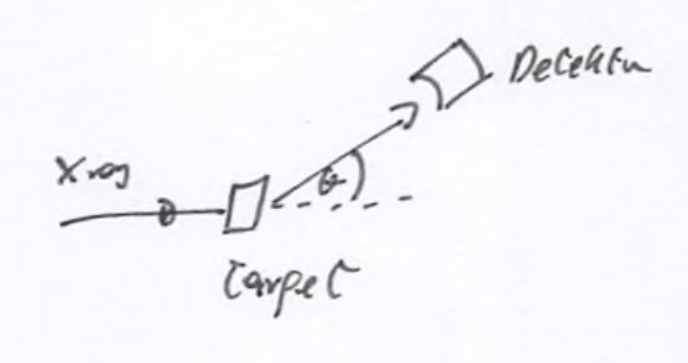
\includegraphics[width=\textwidth]{\currfiledir sketch/compton_setup.png}
    \caption{Versuchsaufbau zur Compton-Streuung}
\end{marginfigure}


 Dieser Effekt kann als Kollision zweier punktförmiger Teilchen 'Photon' und 'Elektron' mit Energie- und Impulserhaltung unter Berücksichtigung des relativistischen Energie-Impulssatzes beschrieben werden. Vor dem Stoß ist das Elektron in Ruhe, danach hat es (relativistische) kinetische Energie. Die Energieerhaltung ist somit
\begin{equation}
    h \nu_0 = h \nu_s + E_{kin} = h \nu_s + \frac{m_0 c^2}{\sqrt{1 - (v/c)^2}} - m_0 c^2 = h \nu_s + (m - m_0) c^2 \quad .
\end{equation}
Eine elektromagnetische Welle hat auch nach klassischem Verständnis einen Impuls. Dieser muss sich also in den Photonen wiederfinden. Der Impuls $\bp$ eines Photons ist 
\begin{equation}
    \bp = \hbar \bk \quad \text{bzw} \quad p = \hbar k = \frac{h}{\lambda} = \frac{h \nu}{c} \quad .
    \label{eq:2_impuls_photon}
\end{equation}
Die Impulserhaltung schreibt sich also als
\begin{equation}
    \hbar \bk_0 = \hbar \bk_s + \bp_e = \hbar \bk_s + \frac{m_0 \boldsymbol{v}}{\sqrt{1 - (v/c)^2}} \quad .
\end{equation}
Man quadriert die Energie- und die Impulsgleichung und setzt sie ineinander ein. Mit den Winkel $\phi$ zwischen Einfalls- und Streurichtung erhält man
\begin{equation}
    \nu_0 - \nu_s = \frac{h}{m_0 c^2} \, \nu_0 \nu_s (1 - \cos \phi)
\end{equation}
bzw. durch Umschreiben nach Wellenlängen die \emph{Compton-Streuformel}
\begin{equation}
    \lambda_s - \lambda_0 =  \lambda_C \, (1 - \cos \phi) \quad \text{mit} \quad
    \lambda_C = \frac{h}{m_0 c} = 2.42 \cdot 10^{-12} m \quad .
\end{equation}
Die Konstante $\lambda_C$ nennt man \emph{Compton-Wellenlänge} des Elektrons.


\begin{marginfigure}
    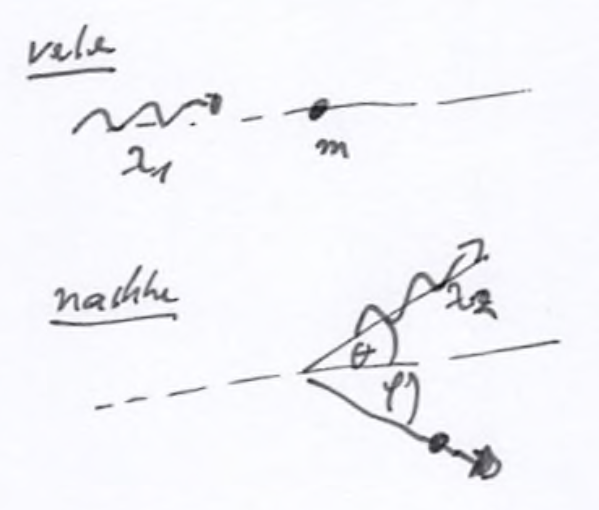
\includegraphics[width=\textwidth]{\currfiledir sketch/compton_vorher_nachher.png}
    \caption{Kollision von Photon und Elektron.}
\end{marginfigure}


 \section{Materiewellen}

 Der Welle-Teilchen-Dualismus funktioniert auch umgekehrt. Wir können nicht nur einer klassischen Welle Teilcheneigenschaften zuschreiben, wie es bei Photonen der Fall ist, sondern wir können auch bei klassischen Teilchen Welleneigenschaften finden. Diese Symmetrieidee hatte Louis de Broglie im Jahre 1924. Ohne experimentelle Belege, rein aus der Analogie zu den 19 Jahre zuvor von Einstein eingeführten Photonen, postulierte er eine heute \emph{de-Broglie-Wellenlänge} genannte Größe, ausgehend von Gl.~\ref{eq:2_impuls_photon}
 \begin{equation}
     \lambda_{dB} = \frac{h}{p} = \frac{h}{m v} = \frac{h}{\sqrt{2 m E_{kin}}} \approx \frac{h c}{E}
 \end{equation}
 wobei im letzten Schritt für relativistische Teilchen angenommen wird, dass ihre Energie $E$ viel größer als die Ruheenergie ist.
 
 
 Lassen Sie uns ein paar Zahlen einsetzen. Ein Elektron, das in einem Kondensator mit einer Potentialdifferenz von \si{1}{V} beschleunigt wird, hat eine Energie von 1~eV und eine Geschwindigkeit von etwa $5.9 \cdot 10^5$ m/s. Das ist schnell für unsere Verhältnisse. Aber für ein Elektron sind sowohl die Energie als auch die Geschwindigkeit klein. Die zugehörige de Broglie-Wellenlänge ist 1.2~nm, ähnlich der Wellenlänge von Röntgenstrahlen und immer noch zehnmal größer als die typischen Abstände in einem Kristallgitter.

 1926 konnten Clinton Davisson und sein Assistent Lester Germer zeigen, dass Elektronen tatsächlich Welleneigenschaften besitzen.
 Ein Elektronenstrahl trifft auf einen Nickelkristall. Die Reflexion zeigt ein Interferenzmuster, das aus der Wellenlänge des Elektrons und dem Gitterabstand des Nickels berechnet werden kann. Letzterer war damals aus der Röntgenbeugung gut bekannt. Davisson erhielt dafür 1937 den Nobelpreis.
 
 \begin{marginfigure}
    \inputtikz{\currfiledir davisson}
    \caption{Beugung eines Elektronenstrahls an einem Nickel-Kristall. Daten aus \cite{Davisson27}.}
\end{marginfigure}


 Mit zunehmender Masse wird die de Broglie-Wellenlänge kleiner. Bei massereicheren Objekten wird es daher schwieriger, Welleneigenschaften zu beobachten. Man kann aber Atome, Moleküle und Proteine durch eine Art Doppelspalt schicken und dann ihre Interferenz beobachten. Einige Forschungsgruppen verfolgen die Idee, kleine Viren mit sich selbst zur Interferenz zu bringen.


 \section{Teilchen im Kasten}

 Materiewellen, also die Welleneigenschaften von Teilchen, haben eine wichtige Konsequenz: Damit sind auch die Energien, die ein Teilchen annehmen kann, quantisiert und nicht mehr kontinuierlich wählbar. So wie ein Lichtstrahl aus einer ganzzahligen Anzahl von Photonen bestehen muss und damit die Energie quantisiert ist, kann ein Teilchen (in sehr vielen Situationen) nur bestimmte Energien annehmen.

 Betrachten wir das einfachste Beispiel: ein Teilchen in einem Kasten. Wir nehmen einen Kasten der Länge $L$ an, in dem sich ein Teilchen befinden soll. Die Wände des Kastens sind undurchlässig. Die beiden anderen Raumrichtungen spielen keine Rolle, es handelt sich also um einen eindimensionalen Kasten. Im klassischen Fall bewegt sich das Teilchen im Kasten mit einer bestimmten Geschwindigkeit und wird an jeder Wand reflektiert. Dabei soll es keine Energie verlieren, so dass sich nur das Vorzeichen der Geschwindigkeit ändert. Die Gesamtenergie bleibt erhalten und kann im klassischen Fall einen beliebigen Wert annehmen.


 \begin{marginfigure}
    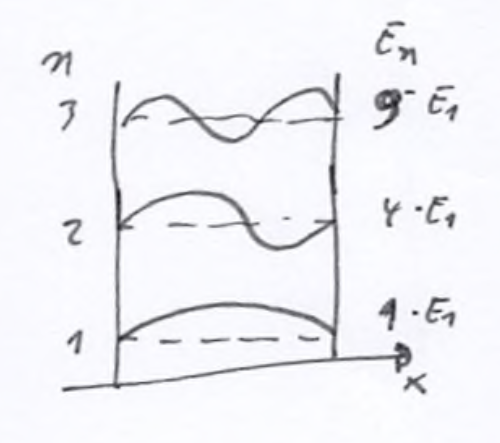
\includegraphics[width=\textwidth]{\currfiledir sketch/Teilchen_im_kasten.png}
    \caption{Teilchen im Kasten: Wellenfunktionen und Energien}
 \end{marginfigure}

Nimmt man jedoch eine Materiewelle zur Beschreibung des Teilchens, so hat diese Welle die de Broglie Wellenlänge $\lambda_{dB}$. Diese Welle wird an den Wänden des Kastens reflektiert und es bilden sich Knoten an den Wänden und eine stehende Welle. Dies ist nur bei bestimmten Wellenlängen $\lambda_n$ möglich
\begin{equation}
    \lambda_n = \frac{2L}{n} \quad \text{mit} \quad n = 1, 2, 3, \dots \quad .
\end{equation}
Die de Broglie-Wellenlänge muss dieser Wellenlänge entsprechen: $\lambda_{dB} = \lambda_n$, woraus sich eine Bedingung für die Geschwindigkeit ergibt
\begin{equation}
    v_n = n \frac{h}{2 L m} \quad \text{mit} \quad n = 1, 2, 3, \dots
\end{equation}
und das Teilchen nur diskrete Energien annehmen kann
\begin{equation}
    E_n = \frac{1}{2} m v_n^2 = n^2 \, \frac{h^2}{8 m L^2} \quad \text{mit} \quad n = 1, 2, 3, \dots \quad .
\end{equation}
Die Energie ist quantisiert 
\begin{equation}
    E_n = n^2 \, E_1\quad \text{mit} \quad E_1 = \frac{h^2}{8 m L^2}  \quad .
\end{equation}
Die $E_n$ werden als Energieniveaus und $n$ als Quantenzahl bezeichnet. Für das Teilchen im Kasten gibt die Quantenzahl die Anzahl der Bäuche der stehenden Welle an.

Was ist passiert? Durch die Einschränkung der Bewegung (engl. confinement) des Teilchens auf den Kasten der Länge $L$ sind diskrete Energieniveaus entstanden. Das Teilchen kann nun nur noch bestimmte Geschwindigkeiten annehmen. Ein freies Teilchen, das sich nicht in einem Kasten befindet, kann weiterhin beliebige Energien annehmen. Die fundamentale Energie ist $E_1 \propto 1/L^2$. Je größer der Kasten, desto näher liegen die Energieniveaus beieinander. Für makroskopische Kästen ist die Quantisierung also nicht mehr erkennbar.



\section{Bohrsches Atommodell}

Im letzten Kapitel haben wir gesehen, wie das Rutherford-Modell den Aufbau eines Atoms beschreibt und damit die Streuexperimente mit Alphateilchen erklärt. Einsteins Vorstellung von Photonen als Lichtquanten erklärt den Photoeffekt, aber die diskreten Linien in den Absorptions- und Emissionsspektren atomarer Gase waren noch nicht verstanden. Eigentlich lag die Idee auf dem Tisch: Wenn Licht nur als Quanten existiert und Atome Licht absorbieren und emittieren, dann muss auch die Energie im Atom quantisiert sein. Das war die Idee von Niels Bohr im Jahr 1913.

Im Bohrschen Atommodell machte er folgende Annahmen
\begin{enumerate} \setlength{\itemsep}{0pt}
    \item Im Rutherford-Modell sind nur bestimmte Bahnen erlaubt, auf denen ein Elektron den Atomkern umkreist. Diese erlaubten Bahnen sind stationär, d.h. für immer stabil. Insbesondere strahlt ein Elektron auf einer solchen Bahn keine Energie ab.
    \item Jede stationäre Bahn hat eine wohldefinierte, diskrete Energie $E_n$. Man kann die Bahnen nach dieser Energie sortieren und so $n$ als Quantenzahl verwenden.
    \item Ein Atom macht einen \emph{Quantensprung}, wenn es von einem stationären Zustand in einen anderen übergeht. Die Energiedifferenz zwischen den beiden Zuständen entspricht der Energie des Photons, das dabei emittiert oder absorbiert wird. Energie kann aber auch in Form von Stößen auf andere Atome übertragen werden.
\end{enumerate}
Für die Energie $h\nu$ der absorbierten oder emittierten Photonen, d.h. für die Frequenz $\nu$ der Linien in den Spektren gilt also
\begin{equation}
    h \nu = \Delta E_{Atom} = | E_f - E_i |
\end{equation}
wenn das Atom zwischen Zuständen mit den Quantenzahlen $i$ nach $f$ wechselt.


Diese Postulate haben weitreichende Konsequenzen
\begin{description}
    \item[Materie ist stabil] Im Grundzustand gibt es keine energetisch niedrigeren Zustände. Das Atom kann seine Energie nicht weiter absenken und bleibt für immer in diesem Zustand.
    \item[Diskretes Spektrum] Die absorbierten oder emittierten Photonen müssen mit ihrer Energie zu den \emph{Abständen} zwischen den Energieniveaus des Atoms passen. Alles andere würde die Energieerhaltung verletzen.
    \item[Emissionsspektrum] In einer Gasentladungsröhre werden die Atome durch Kollisionen untereinander angeregt. Aus einem solchen  angeregten Zustand emittiert das Atom Photonen mit Frequenzen, die den Sprüngen in tiefere Zustände entsprechen.
    \item[Absorptionsspektrum] Damit ein Atom eib Photon mit der Frequenz $ h \nu = | E_f - E_i |$ absorbieren kann, muss es sich im Zustand mit der Quantenzahl $i$ befinden. Im Dunkeln befindet es sich aber früher oder später immer im Grundzustand $i=1$. Absorptionsübergänge gehen daher nur von diesem Zustand aus. Emissionsübergänge führen ebenfalls auf diesen Zustand zurück, aber auch auf viele andere Zustände. Daher sind die Linien in Absorption eine Untermenge der Linien in Emission.
    \item[Elemente] Die erlaubten Bahnen und ihre Energien sind für jedes Element charakteristisch und damit auch die Spektrallinien. 
\end{description}


\section{Energiezustandsdiagramm}

Ein Energieniveau-Diagramm ist ein wichtiges Hilfsmittel, um den Überblick über die Energieniveaus eines Quantensystems und die möglichen Übergänge zwischen den Niveaus zu behalten. Es besteht nur aus einer Achse, der Energie, die vertikal aufsteigend aufgetragen wird. Die horizontale Richtung ist ohne Bedeutung. Die Energieniveaus werden als horizontale Linien gezeichnet und mit ihrer Quantenzahl beschriftet. Das niedrigste Niveau ist immer der Grundzustand, alle anderen sind angeregte Zustände. Übergänge (Quantensprünge) werden als senkrechte Pfeile vom Anfangszustand zum Endzustand gezeichnet.


\begin{marginfigure}
    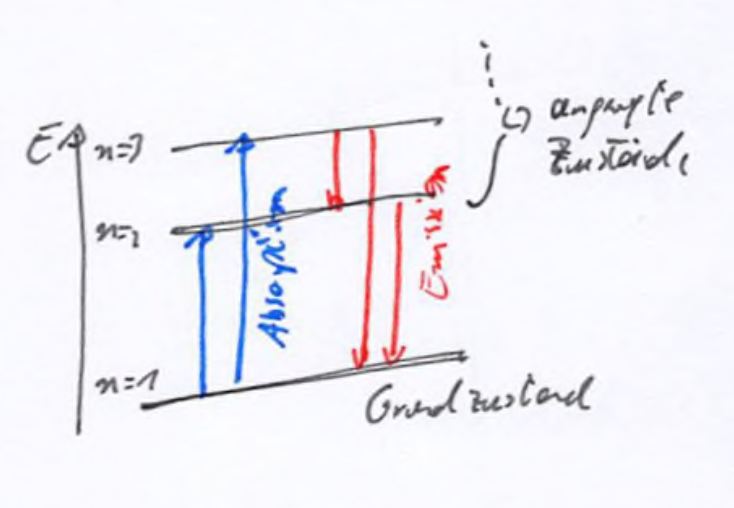
\includegraphics[width=\textwidth]{\currfiledir sketch/diagramm_demo.png}
    \caption{Beispiel eines Energiezustandsdiagramms}
 \end{marginfigure}


\section{Die stationären Zustände des Wasserstoffatoms}

Was können wir über die von Bohr postulierten stationären Zustände sagen? Ein einzelnes Elektron umkreist ein Proton. Sowohl das Elektron als auch das Proton können als Welle oder als Teilchen betrachtet werden. Nehmen wir zunächst an, dass beide Teilchen sind. Dann haben wir ein klassisches Zweikörperproblem. Die Coulombsche Anziehungskraft muss gerade die Zentripetalkraft ergeben, also
\begin{equation}
    \frac{m v^2}{r} = \frac{e^2}{4 \pi \epsilon_0 \, r^2}
\end{equation}
wobei die Ladungen des Elektrons und des Kerns $\mp e$ sind und $m$ die Masse des Elektrons beschreibt. Wir nehmen an, dass der Kern unendlich schwer ist und sich daher in Ruhe befindet. Damit haben wir einen Zusammenhang zwischen der Geschwindigkeit $v$ und dem Bahnradius $r$ des Elektrons, ähnlich wie bei den Bahnen eines Planeten um die Sonne.

Wenn wir das Elektron als Materiewelle auffassen, dann muss der Umfang der Kreisbahn gerade ein ganzzahliges Vielfaches der de Broglie-Wellenlänge sein, damit die Bahn stabil ist, also
\begin{equation}
    2 \pi r = n \lambda_{dB} = n \frac{h}{m v}. \quad \text{mit} \quad n = 1, 2, 3, \dots \quad .
\end{equation}
Damit haben wir zwei Beziehungen zwischen $r$ und $v$, die wir nach dem Bahnradius $r$ auflösen können.
\begin{equation}
    r_n = n^2 \frac{4 \pi \epsilon_0 \, \hbar^2}{m e^2} = n^2 \, a_B \quad .
\end{equation}
Wir haben die häufig verwendete Abkürzung $\hbar = h / (2\pi)$ verwendet und den Bohrschen Bahnradius $a_B$ des Grundzustands mit $a_B = 0.0529$~nm eingeführt. Der Bahnradius wächst quadratisch mit der Quantenzahl. Andere Radien als $r_n$ sind nicht möglich. Dies sind die stationären Zustände des Wasserstoffs im Bohr-Modell.

\section{Energieniveaus im Wasserstoffatom}

Die diesen Bahnradien zugeordneten Energien $E_n$ ergeben sich aus der Summe der kinetischen Energie und der Coulomb-Energie. 
\begin{equation}
    E_n = \frac{1}{2} m v_n^2 - \frac{e^2}{4 \pi \epsilon_0 \, r_n^2}
    = - \frac{1}{n^2} \, \left( \frac{1}{4 \pi \epsilon_0}  \, \frac{e^2}{2 a_B} \right) 
    =  \frac{R_y}{n^2}  
\end{equation}
mit der \emph{Rydberg-Energie} $R_y = h c R_\infty =  - 13.60$eV, und der Rydberg-Konstanten $R_\infty$. Mit steigender Quantenzahl rücken die Zustände energetisch immer näher zusammen und nähern sich der Null. $E=0$ beschreibt ein ruhendes Elektron (kinetische Energie Null), das unendlich weit vom Kern entfernt ist (Coulombpotential Null). Dies ist das freie Elektron.

Das gebundene Elektron-Proton-Paar hat eine niedrigere Energie, weil wir Energie aufwenden müssen, um es in den freien Zustand zu überführen. Daher bezeichnet man $|E_n|$ als \emph{Bindungsenergie}, also die Energie, die in der Bindung steckt. Die Bindungsenergie des Grundzustandes $|E_1|$ wird auch als \emph{Ionisierungsenergie} bezeichnet. Will man ein Elektron aus einem Atom entfernen, also das Atom ionisieren, so muss man diese Energie aufbringen, da sich Atome eigentlich immer im Grundzustand befinden. 

\begin{marginfigure}
    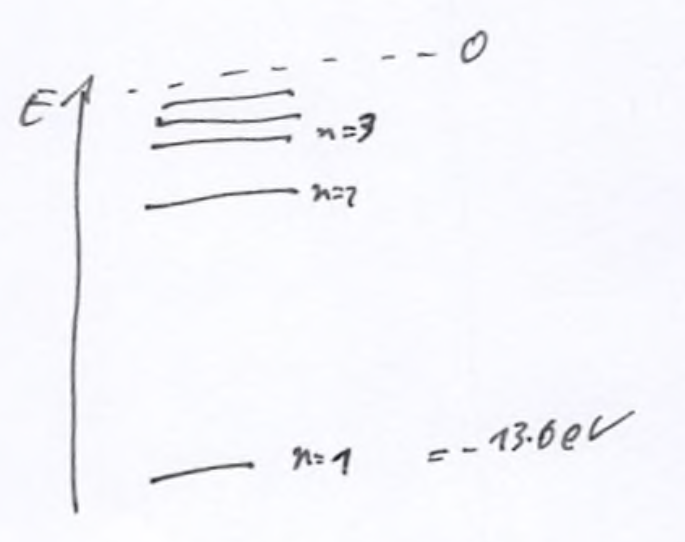
\includegraphics[width=\textwidth]{\currfiledir sketch/Bohr_Energien.png}
    \caption{Zustände des Wasserstoffatoms im Bohr-Modell}
    \label{fig:2_H_zustaende}
 \end{marginfigure}


\section{Quantisierung des Drehimpulses}

Der Drehimpuls $L$ eines klassischen Teilchens auf einer Kreisbahn mit dem Radius $r$ ist $L = m v r$.
Da die Coulombkraft als Zentralkraft kein Drehmoment auf das Teilchen ausüben kann, bleibt der Drehimpuls konstant. Setzt man die oben berechneten Parameter $r_n$ und $v_n$ der Bohr'schen Bahnen ein, so erhält man
\begin{equation}
    L = m v_n r_n = m  \, \frac{n \hbar}{m r_n} \, r_n = n \hbar \quad \text{mit} \quad n = 1, 2, 3, \dots \quad .
\end{equation}
Der Drehimpuls ist also ebenfalls quantisiert und kann nur ganzzahlige Vielfache von $\hbar$ annehmen.

\paragraph*{Nebenbemerkung} Historisch gesehen ist es genau umgekehrt, als ich es hier dargestellt habe (Knight folgend). Bohr postulierte die Quantisierung des Drehimpulses. Die de Broglie Wellenlänge kam erst ca. 10 Jahre später.


\section{Das Spektrum von Wasserstoff}

Abbildung \ref{fig:2_H_zustaende} zeigt das Energiezustandsdiagramm von Wasserstoff im Bohr'schen Modell. Absorptionslinien müssen vom Grundzustand ausgehen. Emissionslinien können aus jedem Zustand stammen, solange die Energie des Atoms abnimmt.

Für den Übergang von $n$ nach $m$ berechnet sich die Frequenz $\nu$ des emittierten ($n > m$) bzw. absorbierten ($n < m$ und damit hier $\nu < 0$) Lichts
\begin{equation}
    h \nu = E_n - E_m  =   \frac{1}{4 \pi \epsilon_0}  \, \frac{e^2}{2 a_B}  \left( \frac{1}{m^2} - \frac{1}{n^2} \right) 
    = R_y  \left( \frac{1}{m^2} - \frac{1}{n^2} \right)  \quad .
\end{equation}
Zum Vergleich mit der Balmer-Formel schreiben wir dies nach Wellenlängen um
\begin{equation}
    \lambda = \frac{\lambda_0}{\frac{1}{m^2} - \frac{1}{n^2}} \quad \text{mit} \quad \lambda_0 = \frac{8 \pi \epsilon_0 h c a_0}{e^2} \approx 91.12 \text{nm} \quad .
\end{equation}
Bei näherer Betrachtung fällt auf, dass die Konstante leicht abweicht. Balmer (und das Experiment) finden $\lambda_0 = 91.18$~nm. Der Grund dafür ist, dass wir bisher die Kernmasse als unendlich angenommen haben. Bei korrekter Berücksichtigung der Kernmasse ändert sich in allen Gleichungen nur die Elektronenmasse $m$ zu einer effektiven Masse $\mu$ mit
\begin{equation}
    \mu = \frac{M m }{M + m}  
\end{equation} 
mit der Kernmasse $M$ bzw. die Rydberg-Konstante $R_M$ für einen Kern der Masse $M$ zu
\begin{equation}
    R_M = \frac{\mu}{m} \, R_\infty \quad .
\end{equation}
Damit findet auch das Bohrmodell die experimentell beobachtete Konstante $\lambda_0 = 91.18$~nm.




\begin{questions}
 \item In diesem und im vorigen Kapitel haben wir die Emissionsspektren atomarer Gase beschrieben und erklärt. In einem Experiment würde man das Licht einer Gasentladungsröhre mit einem Spektrometer beobachten. 
 Der \emph{Franck-Hertz-Versuch} ist technisch einfacher: Man beobachtet periodische Änderungen der Helligkeit entlang der Gasentladungsröhre. Erkläre Sie diese Effekt mit der Quantisierung der atomaren Zustände.
\end{questions}

\section{Wasserstoffähnliche Systeme}

Das Bohr'sche Atommodell funktioniert bis zu gewissen Grenzen recht gut. Sprechen wir zunächst über einen Fall, der gut funktioniert. Im nächsten Abschnitt kommen die Grenzen.

Unter wasserstoffähnlichen Systemen versteht man im allgemeinsten Fall zwei Teilchen, die durch die Coulombkraft aneinander gebunden sind. Neben dem Proton und dem Elektron des Wasserstoffatoms sind dies auch hochionisierte kleine Atome, z.B. \ch{He^+} oder \ch{Li^{2+}}. Entzieht man einem Atom alle Elektronen bis auf eines, so umkreist dieses eine Elektron einen $Z$-fach geladenen Kern. Der Bahnradius ist dann proportional zu $1/Z$, die Zustandsenergie proportional zu $Z^2$, sonst ändert sich nichts. Diese Ionen werden also durch das Bohr'sche Modell gut beschrieben. 

Es funktioniert auch relativ gut für Ionen, die nur ein Elektron plus Edelgaskonfiguration haben, z.B. \ch{Ca^+}. Man kann sich die Edelgashülle zusammen mit dem Kern als effektiv einfach positiv geladenen großen Kern vorstellen. Bei näherer Betrachtung erweist sich diese Größe als problematisch. Sogenannte Rydberg-Zustände in Atomen lassen sich auch als Wasserstoff beschreiben. Hier wird ein einzelnes Elektron zu einer sehr hohen Quantenzahl $n$ angeregt, also sehr weit weg vom Rest des Atoms, der dann wie eine Punktladung aussieht. 

Andere Beispiele sind Muonium (ein Elektron, das ein Antimuon umkreist), Positronium (ein Elektron und ein Positron) oder Exzitonen (gebundene Paare von Elektronen und Löchern in Halbleitern). 

\begin{questions}
    \item Experimentieren Sie mit der Simulation\phet{Neon_Lights_and_Other_Discharge_Lamps} des Neon-Atoms in einer Gasentladungsröhre! Erklären Sie Ihre Beobachtungen.
\end{questions}


\section{Grenzen des Bohr'schen Modells}

Der große Erfolg des Bohrschen Atommodells bestand darin, stabile Materie erklären zu können. Nach dem Rutherford-Modell hätte das Elektron sehr schnell in den Kern fallen müssen. Die Wasserstofflinien konnten erklärt und nicht nur mit der Balmer-Formel ohne Begründung berechnet werden.

Das Problem tritt bei größeren Atomen auf, und Helium ist in diesem Fall schon groß. Das Bohrsche Modell kann die Heliumlinien nicht richtig beschreiben. Das liegt nicht so sehr an den Postulaten von Bohr. Es ist immer noch richtig, dass das Elektron in stationären Zuständen bleibt, die sich nur durch Photonen oder Stöße ändern. Das Problem ist, wie man diese stationären Zustände findet. Die Drehimpulsquantisierung bleibt gültig, aber die Methode mit der de Broglie-Wellenlänge, die den Umfang der Bahn ergeben soll, muss durch etwas Besseres ersetzt werden. Das ist die Quantenmechanik.



\section{Zusammenfassung}

\textit{Schreiben Sie hier ihre persönliche Zusammenfassung des Kapitels auf. Konzentrieren Sie sich auf die wichtigsten Aspekte.}

\vspace*{10cm}


 %--------------------
\printbibliography[segment=\therefsegment,heading=subbibliography]
